%%%%%%%% ICML 2021 EXAMPLE LATEX SUBMISSION FILE %%%%%%%%%%%%%%%%%

\documentclass{article}

% Recommended, but optional, packages for figures and better typesetting:
\usepackage{microtype}
\usepackage{graphicx}
\usepackage{subfigure}
\usepackage{booktabs} % for professional tables
\usepackage{amsmath}
\usepackage{amssymb}
\usepackage{array}
\usepackage{units}
\usepackage{float}
% \usepackage{caption}
% \usepackage{subcaption}
% \usepackage{algorithmicx}
% hyperref makes hyperlinks in the resulting PDF.
% If your build breaks (sometimes temporarily if a hyperlink spans a page)
% please comment out the following usepackage line and replace
% \usepackage{icml2021} with \usepackage[nohyperref]{icml2021} above.
\usepackage{hyperref}

% Attempt to make hyperref and algorithmic work together better:
\newcommand{\theHalgorithm}{\arabic{algorithm}}

\newenvironment{conditions}
  {\par\vspace{\abovedisplayskip}\noindent\begin{tabular}{>{$}l<{$} @{${}={}$} l}}
  {\end{tabular}\par\vspace{\belowdisplayskip}}

\usepackage[accepted]{icml2021}

\icmltitlerunning{Tabular Reinforcement Learning}

\begin{document}

\twocolumn[
\icmltitle{Tabular Reinforcement Learning}

\icmlsetsymbol{equal}{ }

\begin{icmlauthorlist}
\icmlauthor{Dimitrios Kourntidis}{equal}
\icmlauthor{s3841863}{equal}

\end{icmlauthorlist}

\icmlkeywords{Machine Learning, ICML}

\vskip 0.3in
]


\section*{Introduction}
This report investigates the effectiveness of tabular reinforcement learning methods in solving a problem small enough to store it's values in tabular form.
It covers different algorithms like Q-value iteration, Q-learning, SARSA, N-Step and Monte Carlo.
\section{Dynamic Programming} \label{sec:Dynamic}
\subsection{Methodology}
In order to implement the Q-value algorithm some methods were required to be completed first.
Specifically the implementation of the greedy policy (Equation \ref{greedy Q}) and the Q-iteration update (Equation \ref{Dynamic Q Value update}).
\begin{equation}
    % \caption{Algorithm 1}
    \label{greedy Q}
    \pi(s) = arg\,max_a\ Q(s,a)
    % \label{greedyQ}
\end{equation}

\begin{equation}
    \label{Dynamic Q Value update}
    Q(s,a) \leftarrow \sum_{s'}[p(s'|s,a) \cdot (r(s,a,s') + \gamma \cdot max_a\,Q(s',a') )]
\end{equation}
After the implementation of those two methods the Algorithm \ref{Dynamic Programming} was implemented.
 
\begin{algorithm}[h]
    \caption{Q-value iteration (Dynamic Programming)}
    \label{Dynamic Programming}
 \begin{algorithmic}
    \STATE {\bfseries Input:} Threshold  $\eta \in \mathbb{R}^+$
    \STATE {\bfseries Result:} The optimal value function $Q^*(s,a)$
    \STATE {\bfseries Initialization:} $\hat{Q}(s,a) = 0\  \forall s \in S, a\in A$
    \REPEAT
        \STATE  $\Delta \leftarrow 0$.
        \FOR{$each \ s$  $\in$ S }
            \FOR{$each \ \alpha \in $A }
                \STATE $x \leftarrow Q(s,a)$
                \STATE $\hat{Q}(s,a) \leftarrow \sum_{s'}[p(s'|s,a) \cdot (r(s,a,s') + \gamma \cdot max_a\,Q(s',a') )]$
                \STATE $\Delta \leftarrow \text{max}(\Delta,|x - \hat{Q}(s,a)|)$
            \ENDFOR
        \ENDFOR
    \UNTIL{$\Delta < \eta$ }
    \STATE $Q^*(s,a) = \hat{Q}(s,a)$
    \STATE $\pi^*(s) = arg\,maxQ^*(s,a) \; \forall s \in S$
    \STATE {\bfseries Return} $Q^*(s,a)$
 \end{algorithmic}
\end{algorithm}
 
In order to compute the optimal policy, we iterate through each state and action, and choose the action for the next step with a greedy policy.
After each step, we update the Q-value for the corresponding state-action pair, and then compute the maximum error \(\Delta\).
This procedure repeats until \(\Delta < \eta\), where \(\eta\)  is threshold value for convergence.
\subsection{Results}

With algorithm's end we have an action which the agent will choose in each state. With 
This is visible if we compare Figure \ref{fig:Initial State} and Figure \ref{fig:Final State} where for 
each state we have only one desired action which will give the biggest cumulative reward for the beginning state. For this arrangement 
(starting from (0,3) and terminating at (7,3)) the algorithm needs 17 iterations to convergence.
    
\begin{figure}[H]
    \centering
    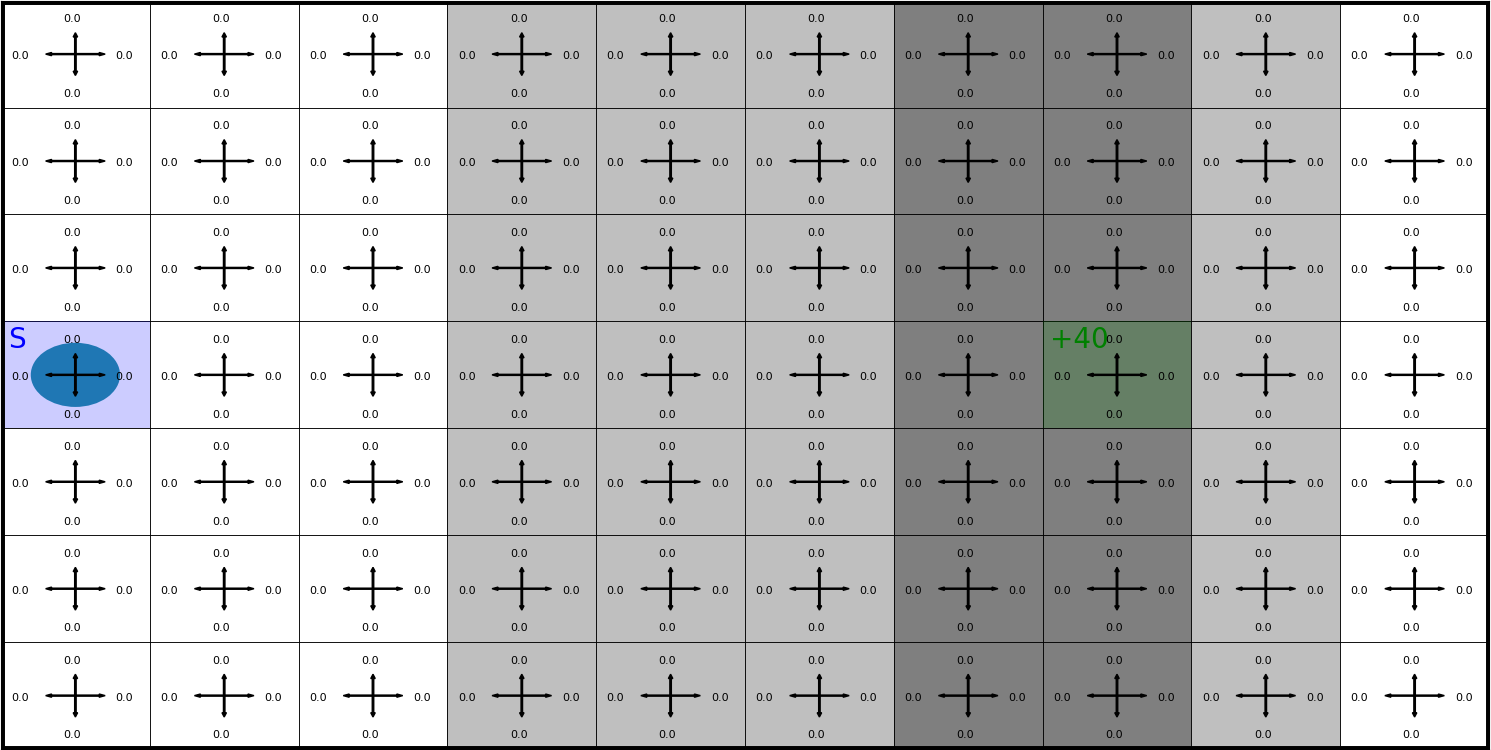
\includegraphics[scale=0.17]{images/Qvalue-initial.png}
    \caption{Q-values at the beginning of the algorithm, each Q(s,a) is initialized with 0 }
    \label{fig:Initial State}
\end{figure}

\begin{figure}[H]
    \centering
    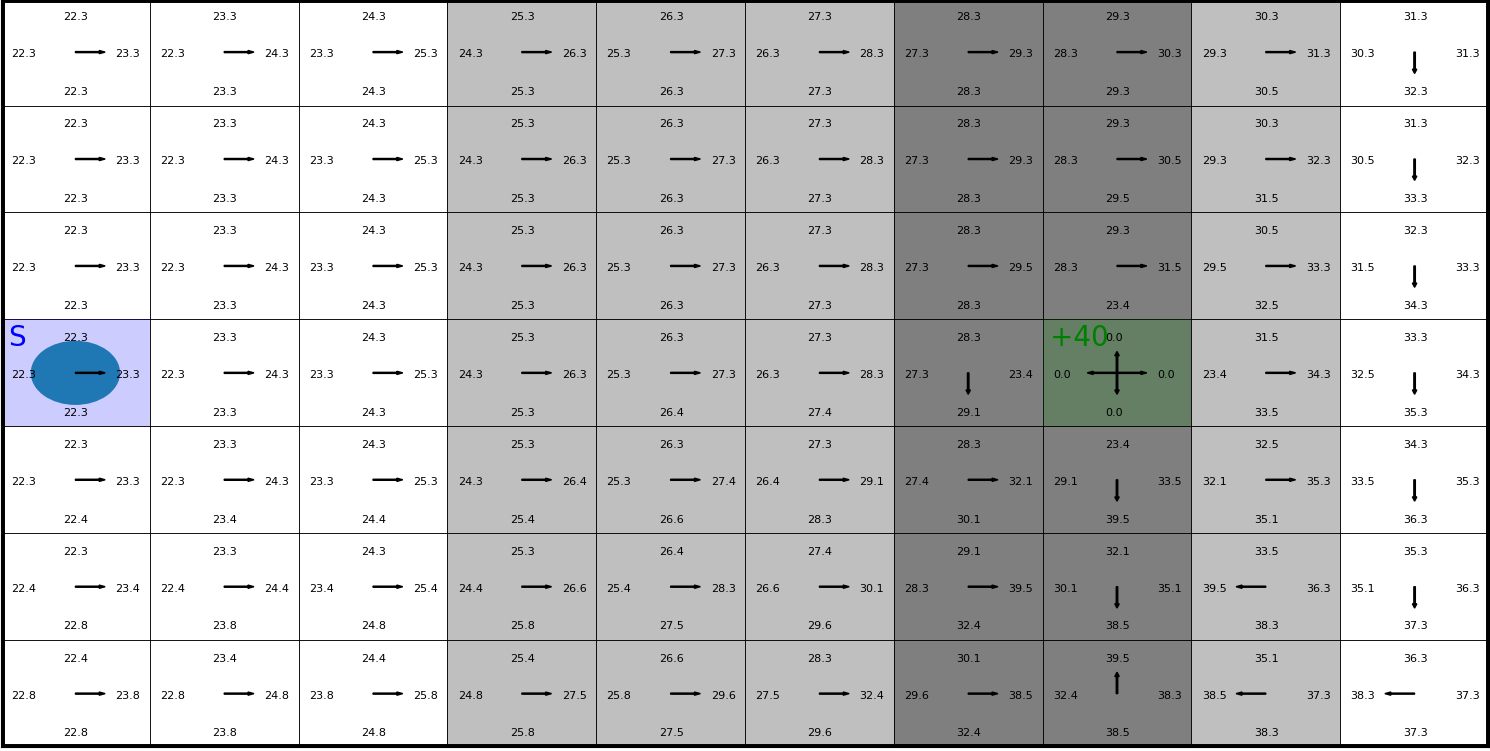
\includegraphics[scale=0.17]{images/Qvalue-last-iteration.png}
    \caption{Q-values after the convergence of the Algorithm \ref{Dynamic Programming}, each state has its optimal action to choose}
    \label{fig:Final State}
\end{figure}
We can also see from Figure \ref{fig:Final State} that $V^*(s=3)=23.3$. That means that the expected reward for our agent when he reaches the terminal state is 23.3

The average reward per timestep is the expected reward that the agent will receive on average in each timestep of the environment.
For this problem the average reward per timestep is  approximately 1.33. This value can be calculated as following:
\begin{equation}
    reward\ per\ timestep = \frac{\sum_{i=1}^{n}\nicefrac{\sum_{j=i}^{steps}r_j}{steps}}{n}
\end{equation}
Where:
\begin{conditions}
    n     &  number of repetitions to get an average value \\
    steps     &  steps needed to reach the terminal state \\   
    r_{j} &  reward for step j
\end{conditions}
The value of $n$ was set to 100.\\

After changing the terminal location to (6,2) we need to compute again the optimal policy. For this terminal state this algorithm
needs 67 iterations to convergence, almost four times more than it needed previously.
Another noticable difference is the $V^*(s=3)$ which now dropped from 23.3 to 19.7.

\section{Exploration} \label{sec:Exploration}
\subsection{Methodology}
In Section \ref{sec:Dynamic}, Dynamic Programming was explored. It is useful when the user has access to the environment. For application 
where there is no access to the model, some exploration is needed to validate that the steps taken so far are the optimal. \\

In this case for the action we have two policies.\\
The $\epsilon$-greedy policy, where a random action is taken with small probability $\epsilon$, otherwise the greedy action is 
selected. With the parameter $\epsilon$ the amount of exploration can be tuned, where $\epsilon \rightarrow 1$ gives random policy
and $\epsilon \rightarrow 0$ gives greedy policy.\\
The second is the Boltzmann policy which can be represented with the Equation \ref{eq:Boltzmann Policy}.
\begin{equation}
    \label{eq:Boltzmann Policy}
    \pi(a|s) = \frac{e^{\nicefrac{\hat{Q}(s,a)}{\tau}}}{\sum_{b\in A}e^{\nicefrac{\hat{Q}(s,b)}{\tau}}}
\end{equation} 

With this equation the action with a higher current value estimate is given a higher probability.
The amount of exploration using this policy can be tuned with the parameter $\tau$. 
When $\tau \rightarrow 0$ the policy becomes greedy and when $\tau \rightarrow \infty$ the policy becomes uniform.
That's because if $\tau \rightarrow \infty$ then the equation \ref{eq:Boltzmann Policy} becomes
$\frac{1}{\sum_{b \in A}1}$. \\

After selecting the action an update have to be performed. To do this we first compute a back-up estimate (Equation \ref{eq:backup Q learning}).
\begin{equation}
    \label{eq:backup Q learning}
    G_t = r_t + \gamma \cdot max_{a'}\, \hat{Q}(s_{t+1}, a')
\end{equation}

Next we update the $\hat{Q}(s_t,a_t)$ values using the Equation \ref{eq:Q learning update}
\begin{equation}
    \label{eq:Q learning update}
    \hat{Q}(s_t,a_t) \leftarrow \hat{Q}(s_t,a_t) + \alpha \cdot [G_t - \hat{Q}(s_t,a_t)]
\end{equation}
Where $\alpha$ denotes the learning rate.\\

Those two equations (Equation \ref{eq:backup Q learning} and Equation \ref{eq:Q learning update}) are used 
to construct the Q-learning algorithm (Algorithm \ref{alg:Tabular Q-learning}). 

\begin{algorithm}[h]
    \caption{Tabular Q-learning}
    \label{alg:Tabular Q-learning}
 \begin{algorithmic}
    \STATE {\bfseries Input:} $\epsilon $, $\alpha \in (0,1]$, $\gamma \in (0,1]$, total budget
    % \STATE {\bfseries Initialization:} $\hat{Q}(s,a) = 0\  \forall s \in S, a\in A$
    % \REPEAT
    \STATE $\hat{Q}(s,a) \leftarrow 0,\ \forall s \in S, a \in A$
    \STATE $s \sim p_0(s)$
        \WHILE{$budget$}
        \STATE $a \sim \pi(a|s)$
        \STATE $r,s' \sim p(r,s'|s,a)$
        \STATE $\hat{Q}(s,a) \leftarrow \hat{Q}(s,a) + \alpha \cdot [G_t - \hat{Q}(s,a)]$
        \IF { s' is terminal}
        \STATE $s \sim  p_0(s)$
        \ELSE 
        \STATE $s \leftarrow s'$
        \ENDIF
        \ENDWHILE
    
    \STATE {\bfseries Return} $\hat{Q}(s,a)$
 \end{algorithmic}
\end{algorithm}
 
After the implementation of the Q-learning algorithm an experiment run to examinate both $\epsilon$-greedy policy and Boltzmann policy using 
different values for $\epsilon$ and $\tau$.

\subsection{Results}
The experiment run for 50,000 timestep and was averaged over 50 repetitions in order to get smoother figure. The results can be observed in Figure \ref{fig:Exploration}

    \begin{figure}[H]
        % \centering
        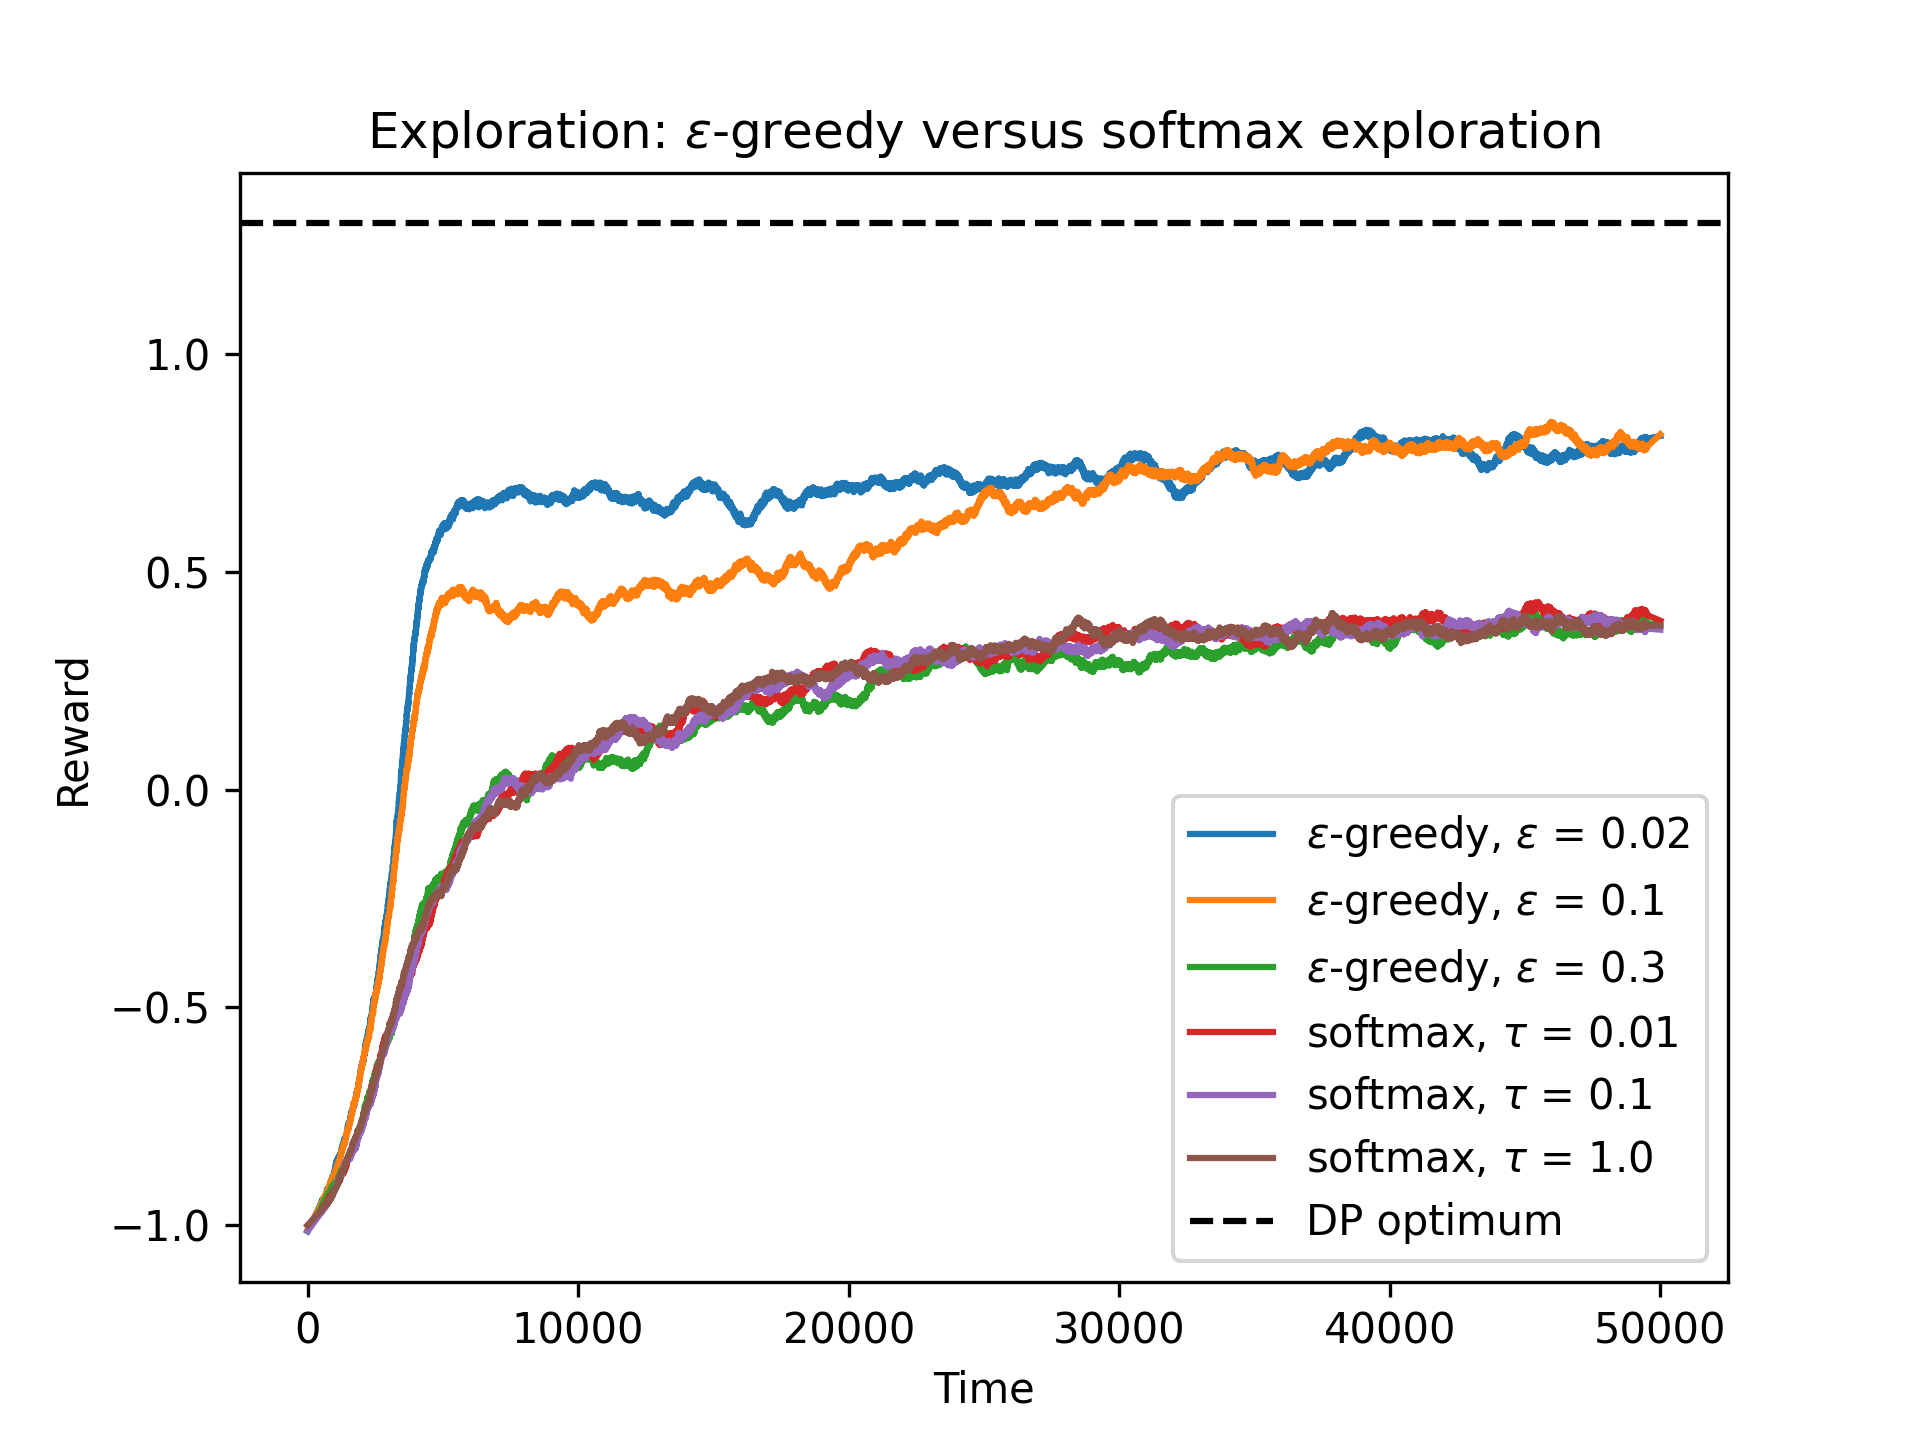
\includegraphics[scale=0.6]{images/exploration.png}
        \caption{Reward per timestep using multiple values for $\epsilon$ and $\tau$ }
        \label{fig:Exploration}
    \end{figure}

From the plot it can be observed that neither policy ($\epsilon$-greedy and Boltzmann) reaches the performance of 
the Dynamic Programming and that is because under Dynamic Programming each action is the optimal one, where now there is the 
possibility of exploration. It can also be seen that $\epsilon$-greedy performs better than the Boltzmann policy, exepction to than is 
$\epsilon = 0.3$. In my opinion that's because the probability of a random choice is bigger than that of the other two choices. 
The method that I prefer is the $\epsilon$-greedy with the $\epsilon = 0.02$ because it converges faster than the other methods.

\section{Back-up: On-policy versus off-policy target} \label{sec:Policy}
\subsection{Methodology}
In this section the way of the back-up will be studied. SARSA will be implemented to see how on-policy behave versus an off-policy (Q-learning).\\
For SARSA the action selection is the same with the Q-learning.
The difference of between on-policy and off-policy is that the first plugs in the value of the best action at the next state and the second uses the value from the action it actually takes.

That leads to the following two equations:

\begin{equation}
    G_t = r_t + \gamma \cdot \hat{Q}(s_{t+1},a_{t+1})
    \label{eq:Sarga G_t}
\end{equation}

\begin{equation}
    \hat{Q}(s_t,a_t) \leftarrow \hat{Q}(s_t,a_t) + a \cdot [G_t - \hat{Q}(s_t,a_t)]
\end{equation}

With those equations, we can construct the Tabular SARSA algorithm.

\begin{algorithm}[h]
    \caption{Tabular SARSA}
    \label{alg:Tabular SARSA}
 \begin{algorithmic}
    \STATE {\bfseries Input:} $\epsilon $, $\alpha \in (0,1]$, $\gamma \in (0,1]$, total budget
    
    \STATE $\hat{Q}(s,a) \leftarrow 0,\ \forall s \in S, a \in A$
    \STATE $s \sim p_0(s)$
    \STATE $a \sim \pi(a|s)$
        \WHILE{$budget$}
        \STATE $r,s' \sim p(r,s'|s,a)$
        \STATE $a' \sim \pi(a'|s')$
        \STATE $\hat{Q}(s,a) \leftarrow \hat{Q}(s,a) + \alpha \cdot [G_t - \hat{Q}(s,a)]$
        \IF { s' is terminal}
        \STATE $s \sim  p_0(s)$
        \STATE $a \sim \pi(a|s')$
        \ELSE {
        \STATE $s \leftarrow s'$
        \STATE $a \leftarrow a'$ }
        \ENDIF
        \ENDWHILE
    
    \STATE {\bfseries Return} $\hat{Q}(s,a)$
 \end{algorithmic}
\end{algorithm}

After the implementation of the SARSA algorithm an
experiment run  to compare on-policy and off-policy using multiple values for $\alpha$.

\subsection{Results}
After 50,000 timesteps we get the results that can be seen in Figure \ref{fig:SARSA} which were averaged over 50 repetitions.
\begin{figure}[h]
    \centering
    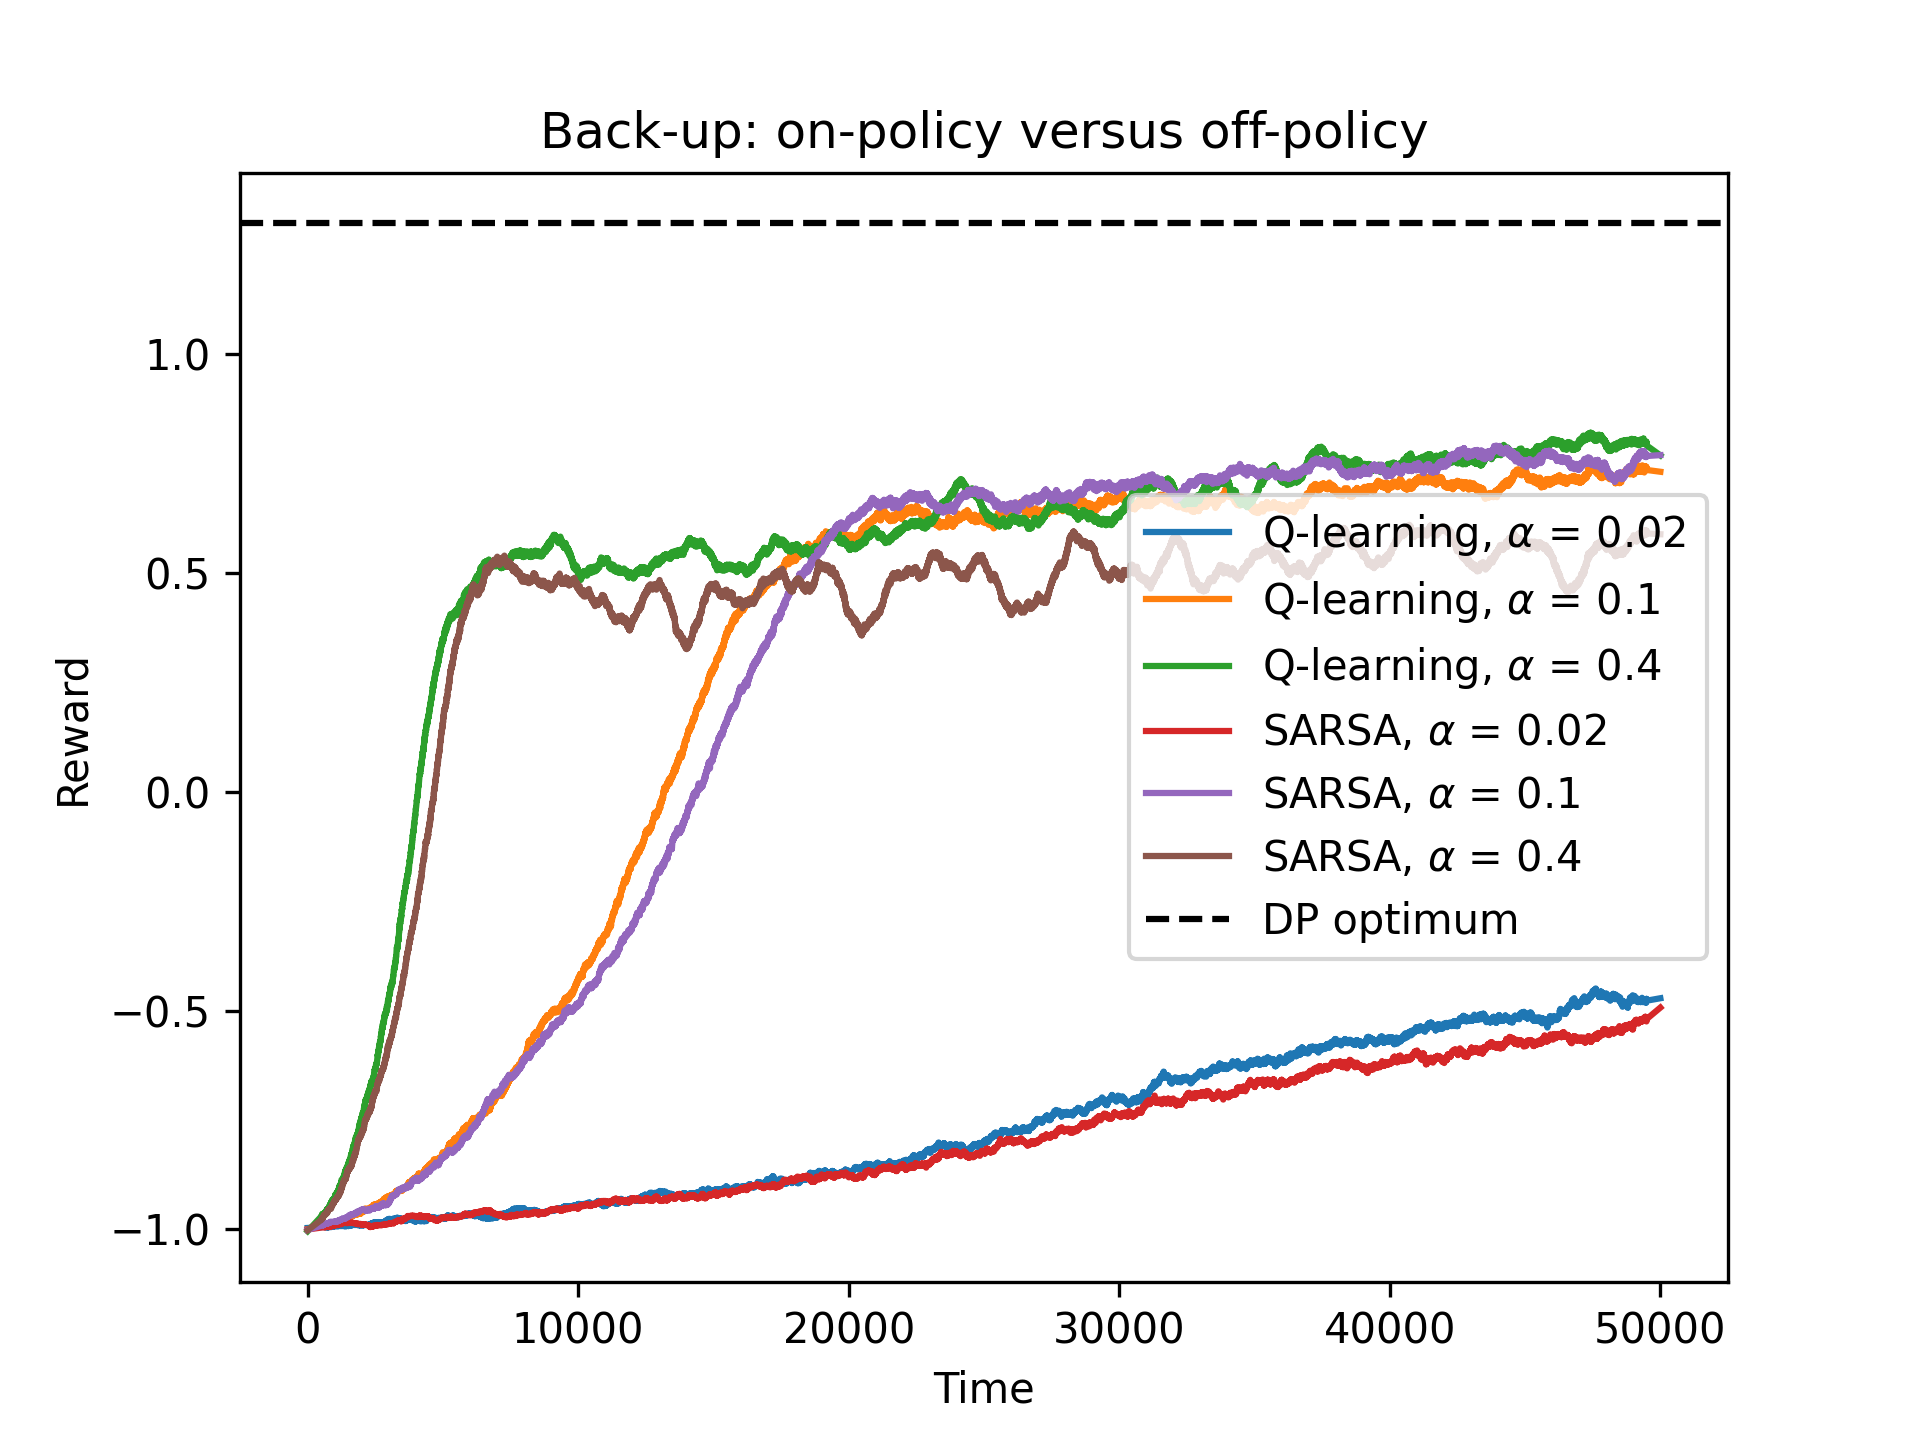
\includegraphics[scale = 0.55]{images/on_off_policy.png}
    \caption{Reward per timestep using multiple values a for both Q-learning and SARSA}
    \label{fig:SARSA}
\end{figure}

Both SARSA and Q-learning with $a = 0.4$ have the steepest plots, and they have the best performance for about 20,000 timesteps. After that the performance of the brown plot remains almost the same on average
while green, orange and purple plots continue to improve. Finally, both SARSA   and Q-learning with $a = 0.02$ improve very slow but steadily.

\section{Back-up: Depth of target}
\subsection{Method}
In this section the depth of the back-up. So far the depth was 1 and now n-step  algorithms  will be examined.
The n-step Q-learning computes the target following the Equation \ref{eq:Depth Target G}.

\begin{equation}
    G_t = \sum_{i=0}^{n-1}(\gamma)^i \cdot r_{i+1} + (\gamma)^n*max_a Q(s_{t+n},a)
    \label{eq:Depth Target G}
\end{equation}
Then we have the tabular update we had in Equation \ref{eq:Q learning update}. 
This formulates the n-step Q-learning that can be seen in Algorithm \ref{alg:Tabular n-step Q-learning}

\begin{algorithm}[h]
    \caption{Tabular n-step Q-learning}
    \label{alg:Tabular n-step Q-learning}
 \begin{algorithmic}
    \STATE {\bfseries Input:} $\epsilon \in (0,1]$, $\alpha \in (0,1]$, $\gamma \in (0,1]$, total budget, maximum episode length T , target depth n
    
    \STATE $\hat{Q}(s,a) \leftarrow 0,\ \forall s \in S, a \in A$
    % \STATE $a \sim \pi(a|s)$
    \WHILE{$budget$}
        \STATE $s_0 \sim p_0(s)$
        \FOR{$t = 0 ...(T-1)$}
            \STATE $a_t \sim \pi(a|s_t)$
            \STATE $r_t,s_{t+1} \sim p(r,s'|s_t,a_t)$
            \IF {$s_{t+1}$ is terminal}
                \STATE \textbf{break}
            \ENDIF
        \ENDFOR
        \STATE $T_{ep} \leftarrow t+1$
        \FOR{$t = 0 ... (T_{ep}-1)$}
            \STATE $m = min(n,T_{ep}-t)$
            \IF {$s_{t+m}$ is terminal }
                \STATE $G_t \leftarrow \sum_{i=0}^{m-1}(\gamma)^i \cdot r_{t+i}$
            \ELSE{\STATE $G_t \leftarrow \sum_{i=0}^{m-1}(\gamma)^i \cdot r_{t+i} + (\gamma)^m \cdot max_a\,\hat{Q}(s_{t+m},a)$}
            \ENDIF
            \STATE $\hat{Q}(s_t,a_t) \leftarrow \hat{Q}(s_t,a_t) + a \cdot [G_t - \hat{Q}(s_t,a_t)] $
        \ENDFOR
    \ENDWHILE
    
    \STATE {\bfseries Return} $\hat{Q}(s,a)$
 \end{algorithmic}
\end{algorithm}


We can also sum all the rewards that accumulated in the episode, instead of going until the n-step. That gives us the Monte Carlo approach.
In this case the target becomes the following.
\begin{equation}
    G_t = \sum_{i=0}^{\infty}(\gamma)^i \cdot r_{t+i}
\end{equation}
The update remains the same as before, now we have slightly different algorithm

\begin{algorithm}[h]
    \caption{Tabular Monte Carlo reinforcement learning.}
    \label{alg:Tabular Monte Carlo reinforcement learning.}
 \begin{algorithmic}
    \STATE {\bfseries Input:} $\epsilon \in (0,1]$, $\alpha \in (0,1]$, $\gamma \in (0,1]$, total budget, maximum episode length T
    
    \STATE $\hat{Q}(s,a) \leftarrow 0,\ \forall s \in S, a \in A$
    % \STATE $a \sim \pi(a|s)$
    \WHILE{$budget$}
        \STATE $s_0 \sim p_0(s)$
        \FOR{$t = 0 ...(T-1)$}
            \STATE $a_t \sim \pi(a|s_t)$
            \STATE $r_t,s_{t+1} \sim p(r,s'|s_t,a_t)$
            \IF {$s_{t+1}$ is terminal}
                \STATE \textbf{break}
            \ENDIF
        \ENDFOR
        % \STATE $T_{ep} \leftarrow t+1$
        \FOR{$t = t ... 0$}
            \STATE $G_i \leftarrow r_i + \gamma \cdot G_{i+1}$
            \STATE $\hat{Q}(s_i,a_i) \leftarrow \hat{Q}(s_i,a_i) + a \cdot [G_i - \hat{Q}(s_i,a_i)] $
        \ENDFOR
    \ENDWHILE
    
    \STATE {\bfseries Return} $\hat{Q}(s,a)$
 \end{algorithmic}
\end{algorithm}


\subsection{Results}
After implementing both Monte Carlo and n-step Q-learning algorithms, an experiment run for 50,000 timesteps as before.
In this experiment different values for n were examined as well as the performance of Monte Carlo.

\begin{figure}[h]
    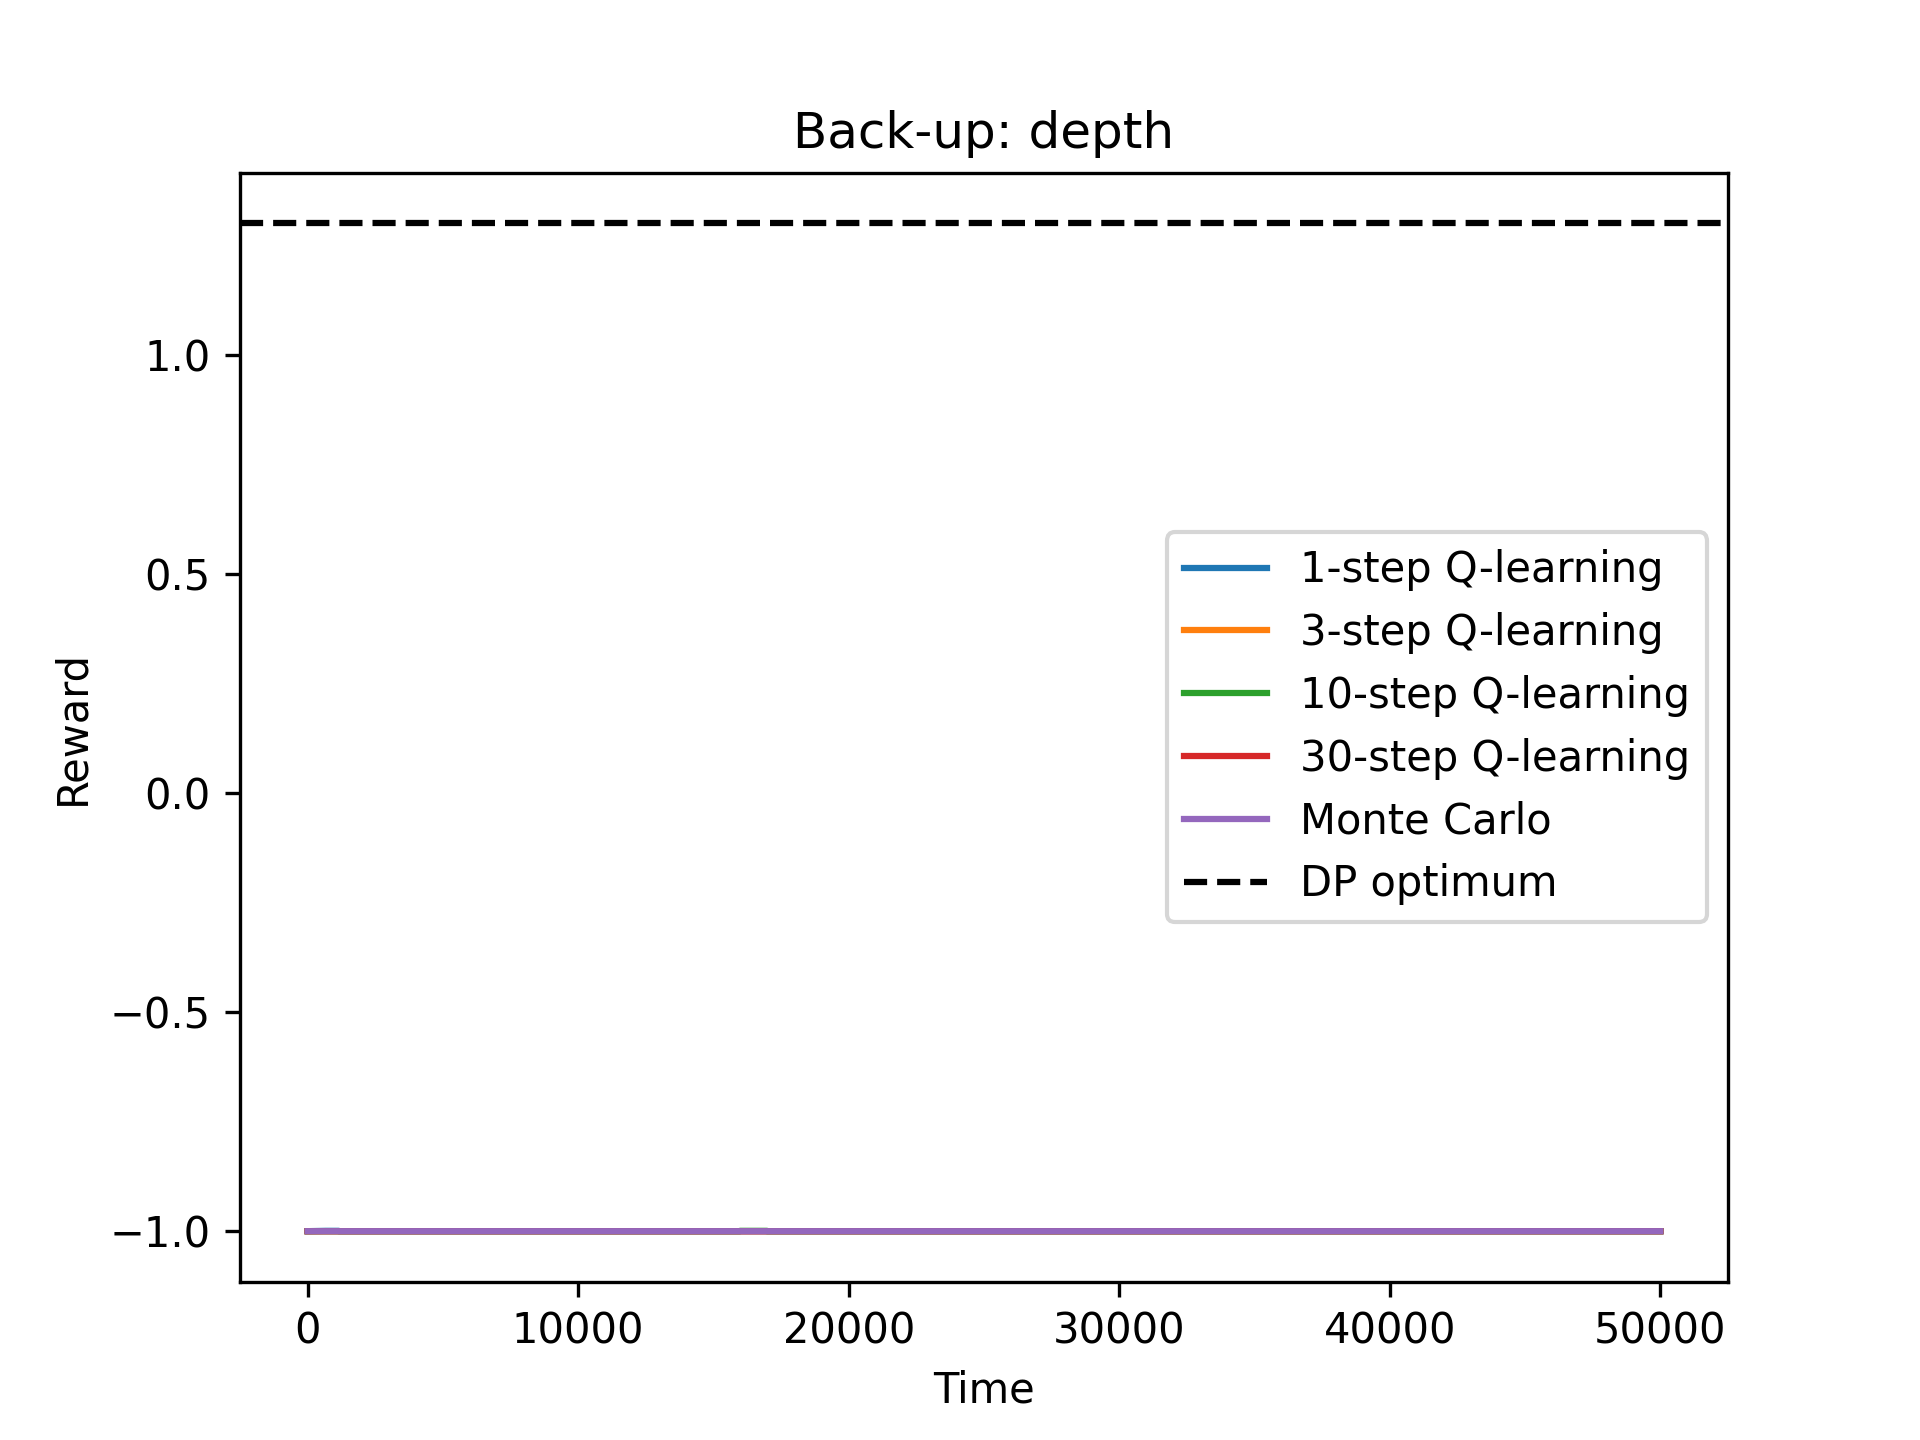
\includegraphics[scale=0.5]{images/depth.png}
    \caption{Average reward per timestep using 1,5,10 and 30 steps}
    \label{fig:katastrofi}
\end{figure}

Having the results in Figure \ref{fig:katastrofi} the average reward stays at -1 which mean the agent never reached the target.  










\section{Reflection}
After many experiments some conclusions can be made. First it is visible that neither algorithm reached the performance of Dynamic Programming.
That's because with Dynamic Programming there is the ability to traverse all possible state-actions and choose the optimal 
action each time.  Although Dynamic Programming creates the best policy, in can be computationally expensive as it was shown  in Section \ref{sec:Dynamic} when the terminal stated
changed. \\

In Section \ref{sec:Exploration} two exploration methods were examined, $\epsilon$-greedy and softmax. For the exploration method I prefer the softmax. $\epsilon$-greedy is less likely to take a random action in order to explore.
If no exploration happen then it is possible that the best policy will not be explored and the agent won't have a better option because he will be stuck in local optimum rather the global

After exploration methods in Section \ref{sec:Policy} two different back-up policies were studied. On-policy and off-policy.
Off-policy algorithms such Q-learning create their policy with greedy selection independently the action the agent made. 
On-policy on the other hand create their policy based on the action they took \cite{sagar_2020}. One problem that on-policy has is The
amount of steps needed to converge because the target policy is not updated each time with the optimal values \cite{Plaat_2022}.

Studying those algorithms gave a great inside what are some solution when the problem is small enough
to fit in a table. The algorithm studied will not work when the state-space is high-dimensional. 
This is also known as the curse of dimentionality.
We can overcome this issue   using deep learning, instead of trying to find the correct action, we try to approximate it.

\bibliography{main}
\bibliographystyle{icml2021}

\end{document}
